\chapter{Applicazione mobile}
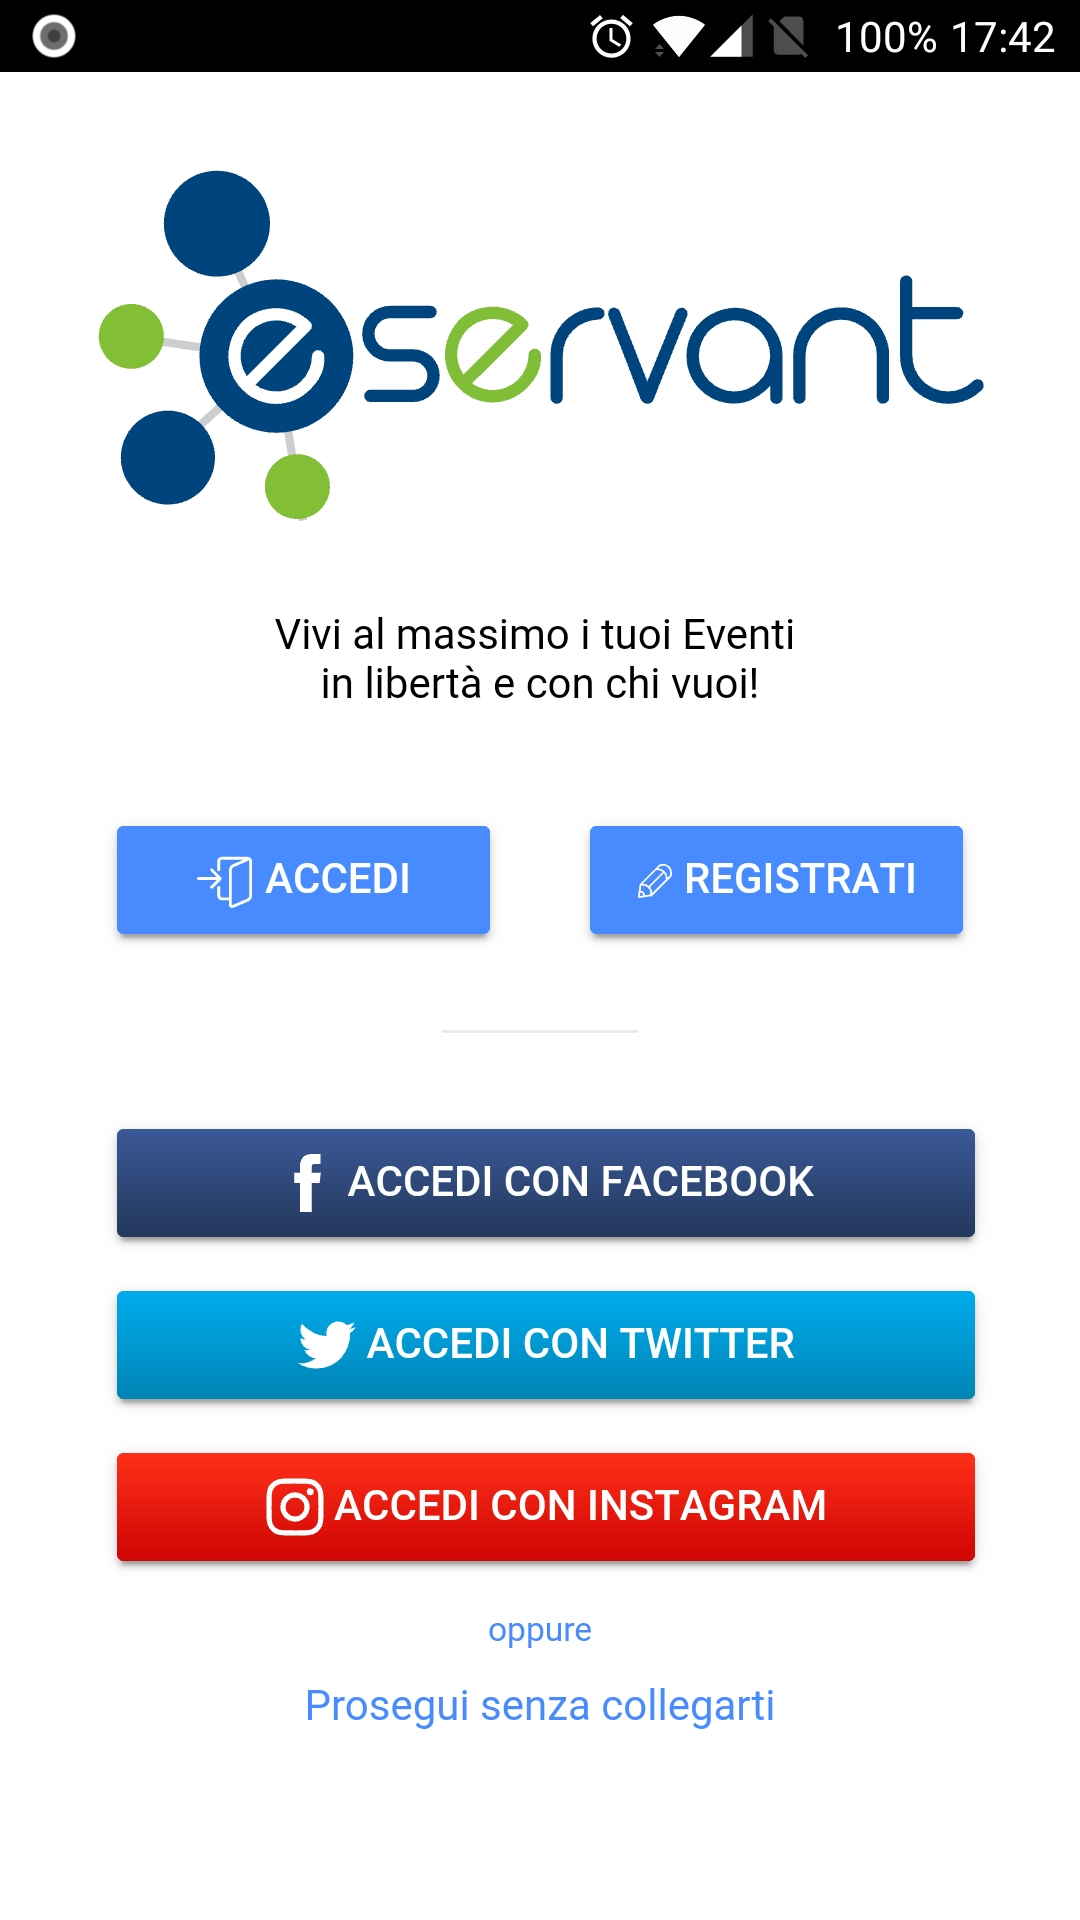
\includegraphics[scale=0.15]{img/cap2/1}\\
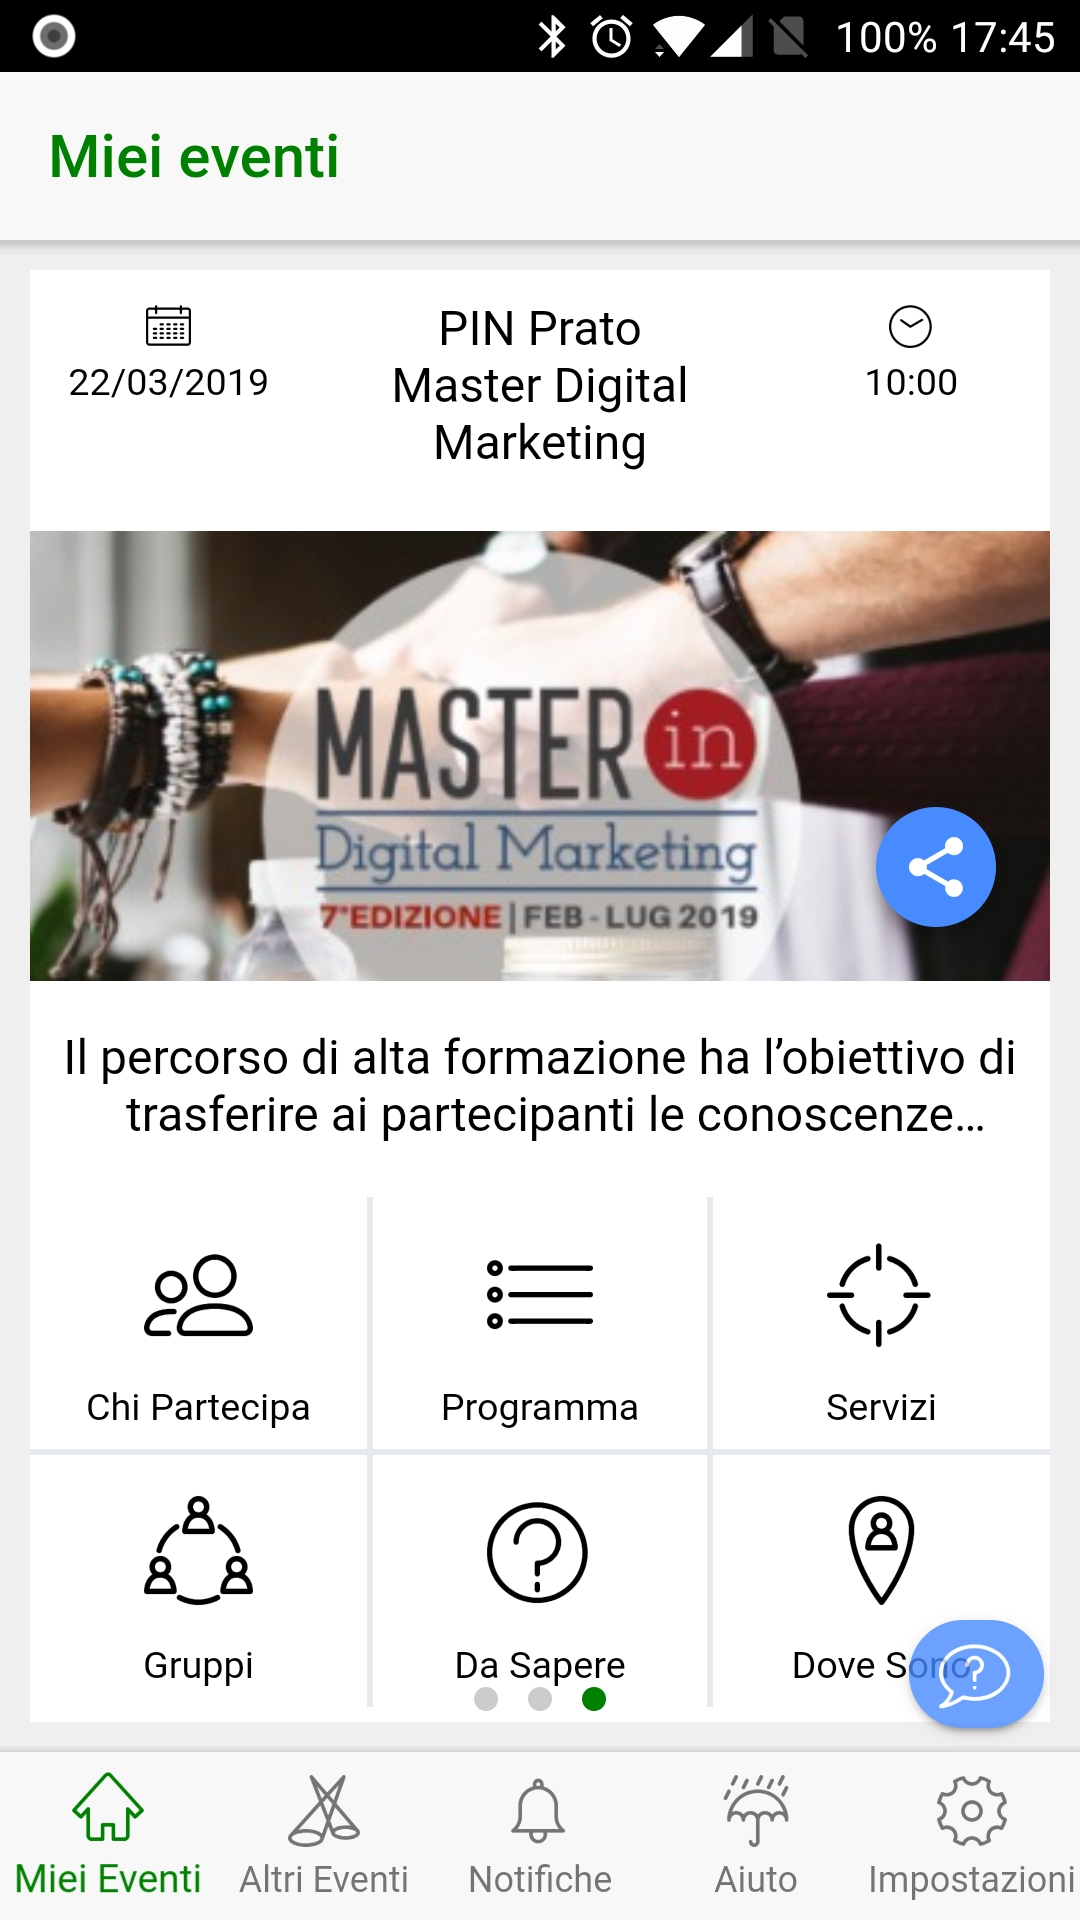
\includegraphics[scale=0.15]{img/cap2/2}\\

L’interfaccia della piattaforma eSERVANT verso gli utenti finali è come da progetto una APP per mobile.
Per questo insieme a Sintra Consulting s.r.l. siamo andati a disegnare in modo molto avanzato tutte le interfacce andando a quadrare requisiti di sistema/casi di uso con mockup montati all’interno di una vera e proprio demo dell’APP finale attesa.
Tale strumento ci ha permesso di valutare non solo la user experience degli utenti, ma anche di poter fornire agli sviluppatori uno strumento specifico sul quale andare a traguardare la loro attività.
Tutte le slide sono state montate e condivise tra tutti i partner del progetto all’indirizzo https://share.proto.io/U2B8EV/, anche se per motivi di praticità non sono state sviluppate tutte le articolazioni della stessa, ma solo le funzioni di maggior impatto e complessità.
Il prototipo di APP è quindi stato creato andando a realizzare slide sui cinque temi di fondo:
\begin{itemize}
\item presentazione e riconoscimento;
\item gestione evento e socialità;
\item gestione delle funzioni di aiuto;
\item gestione delle funzioni di mobilità;
\item gestione delle funzioni di navigabilità e mappe;
\item gestione del proprio profilo.
\end{itemize}

\section{Framework Ionic}
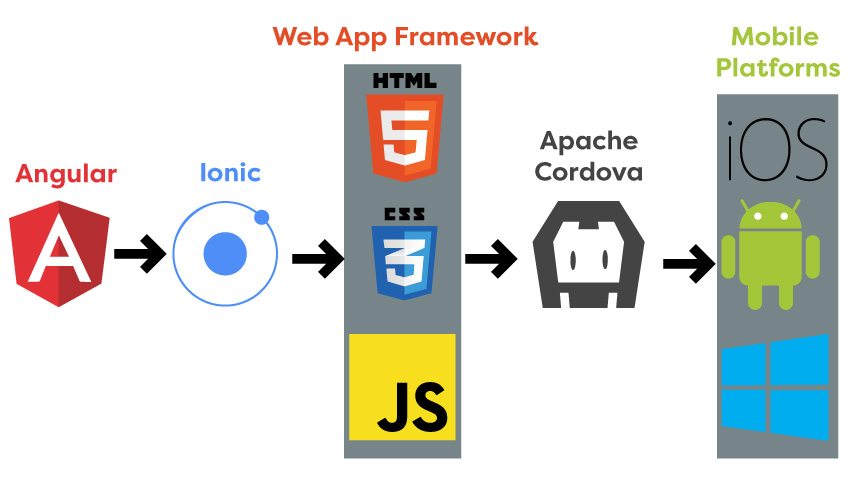
\includegraphics[scale=0.50]{img/cap2/angular-ionic}\\
Ionic è un HTML5 SDK lanciato nella sua prima versione nel 2013 e progettato per essere la base per lo sviluppo di app mobili ibride. 
Sviluppare un app mobile ibrida significa scrivere un unico code base per i due OS più famosi: IOS e Android.

La struttura di Ionic è costituita da Angular, Apache Cordova (ex-PhoneGap) e SASS. Ciò consente la creazione di applicazioni mobili ricche di funzionalità che utilizzano esclusivamente tecnologie web.
\paragraph{}
\textit{Angular}

Angular è un framework web open source creato da Google ed è il successore di AngularJS (primissima versione).
Angular permette ai developer di costruire applicazione fruite nel web, su piattaforme mobile o desktop. 
Angular capisce solo TypeScript dato che il framework è stato proprio scritto in Typescript. 

Elementi positivi emersi sviluppando in Ionic:
\begin{itemize}
    \item essendo tra i più famosi web framework, la \textbf{velocità di sviluppo} è un aspetto caratterizzante di Ionic
    \item \textbf{semplice} da capire
    \item supporta il \textbf{live reload} permettendo così al developer di vedere immediatamente le modifiche direttamente sul dispositivo mobile.
\end{itemize}
    
Elementi negativi emersi:
\begin{itemize}
    \item l'accesso alle funzioni native tramite Cordova è \textbf{limitato}. Non è assolutamente paragonabile alle API native dell'OS.abilità e mappe;
    \item \textbf{instabilità} nell'accesso nativo. Generalmente le librerie Cordova non sono allineate con le ultime API rilasciate da Android/IOS.
\end{itemize}

\paragraph{}

\textit{Apache Cordova, ex-PhoneGap e futuro Capacitor}

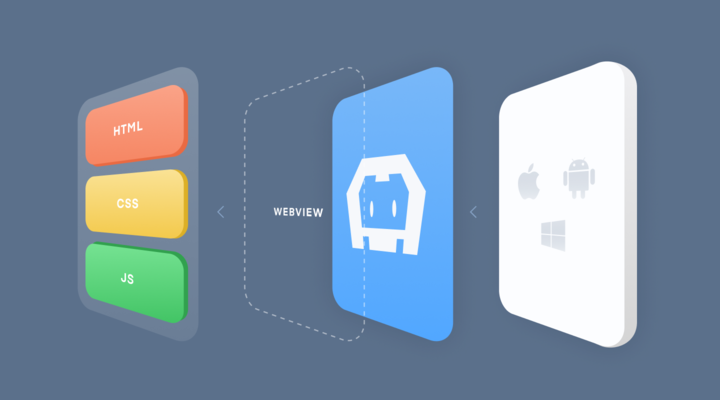
\includegraphics[scale=0.50]{img/cap2/cordova}\\
TODO: descrizione cordova

\paragraph{}
\textit{SASS}

TODO: descrizione SASS

\subsection{NgRx gestore stato}

TODO: descrizione ngrx + flow

\subsection{Android}
TODO:

\subsection{IOS}
TODO:

\section{Social login}
Al primo accesso all'APP eServant è necessario dare il consenso per almeno uno dei seguenti social:
\begin{itemize}
\item Facebook
\item Instagram
\item Twitter
\end{itemize}

Altrimenti viene data la possibilità di fare un accesso privato tramite username e password.
L'autenticazione verso i social network sopra citati avviene tramite protocollo OAuth2.0.

Il framework di autorizzazione OAuth 2.0 abilita un'applicazione di terze parti a ottenere un accesso limitato a un servizio HTTP, attivo
per conto di un proprietario di risorse orchestrando un'inerazione di approvazione tra il proprietario della risorsa e il servizio HTTP.
Questa specifica sostituisce e obsoleta il protocollo OAuth 1.0 descritto in RFC 5849.

OAuth 2.0 flow 

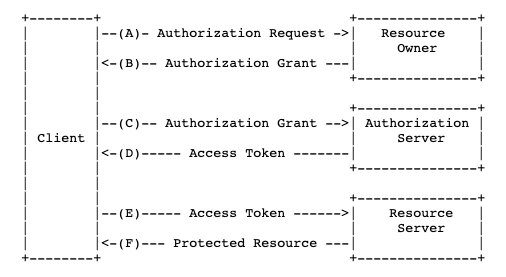
\includegraphics[scale=0.60]{img/cap2/oauth20-1}\\

\textbf{Attori}

\textit{resource owner}: un'entità in grado di approvare l'accesso a una risorsa protetta.

\textit{authorization server}: il server che invia i token di accesso al client dopo essere stato autorizzato
dal resource owner

\textit{resource server}: il server che ospita le risorse protette. Il resource Server è in grado di accettare
e rispondere alle richieste di risorse protette utilizzando i token di accesso.

\textit{client}: un'applicazione che fa richieste di risorse protette per conto di
proprietario di risorse e con la sua autorizzazione. Il termine "client"
non implica particolari caratsteristiche di implementazione (l'applicazione può essere eseguita
su un server, un client web o altri dispositivi).

\section{Geolocalizzazione}
\subsection{iBeacon}
\subsection{QRcode}
\subsection{GPS}
\section{Navigazione (mappe intelligenti)}
\section{Chatbot (DialogFlow)}
